\chapter{A gentle introduction}

This chapter is a gentle introduction to probability. To do statistics
we will need to introduce some mathematical tools. These tools might
initially seem overly formal and un-necessary. My goal in this chapter
is to introduce you to some central concepts in an intuitive way and
motivate the more rigorous definitions that will come later. It is
therefor important that you understand the concepts and examples of
this chapter. If you are having trouble with anything, discuss it with
your peers, post on Piazza, or ask a question in class. If the examples
in this chapter confuse you, you are likely to have a hard time with
the remainder of the class.

\section{Probability and fair bets}

One intuitive way of thinking about probability problems is in terms
of the {\em fair price of a bet}.

Let's start with a very simple example. Suppose I flip a fair coin.
If the coin falls ``heads'' I give you a dollar, if it falls ``tails''
I give you two dollars. What is the fair price for taking part in the
game?

The fair price is the one which, over the long term, will neither
increase nor decrease your wealth. The fair price in this case is
dollar and fifty cents.

Why?

Because if you pay me 1.5 dollars on each turn, then you will either
lose 50 cents (if the outcome is ``head'') or win 50 cents (if the
outcome is ``tails''). As heads and tails have equal chance, the net
result is zero.

A slightly more formal way of saying the same thing is that we have
two outcomes, each with probability $1/2$, so the {\em expected value}
of the game is 
\[
\frac{1}{2} 1 + \frac{1}{2} 2 = 1.5
\]

The {\bf expected value} or {\bf expectation} is the {\em long term
  average of a large number of independent experiments.} Here an
``experiment'' is a single coin toss. The fact that the expectation is
$1.5$ is equivalent to the fact that in a very long sequence of coin
flips we expect the number of ``Heads'' to be close to the number of
``Tails''. This is called the ``law of large numbers''

\iffalse
Note that it is {\em not} reasonable to assume that the number of
Heads is {\em equal} to the number of Tails, which is impossible for a
sequence of odd length. It is also not reasonable that the difference
between the number of Heads and the Number of tails be 1, as in the
sequence $HTHTHTHTHTHT \ldots$. What can we expect to be the magnitude
of the difference between the numbers of H's and T's? 
\fi

Hopefully, you find this example trivial. Indeed, if all of the
problems we encountered in this course were as simple, there would be
no need for formal math. However, as you'll see in the following
sections, even seemingly simple problems can have unintuitive answers.

The examples we will go through share a common theme; we will describe
a game of chance between the ``player'' and the ``house'' of the following form:
\begin{enumerate}
\item The player buys from the house a ticket to participate in the
  game. We will discuss this price in detail below.
\item The house uses some randomization device: a coin flip, a die
  toss, a spin of a roulette wheel etc. to generate an {\em
    outcome}. All of the outcomes are equally probable. Thus, if there
  are $k$ possible outcomes, each has probability $1/k$.
\item The house pays the player according to the outcome and a
  predefined table.
\end{enumerate}

Both sides know the payment corresponding to each outcome. The
question is what is the ``fair'' price for the ticket.

\section{Event Trees}

Event trees are simple figures that can aid in reasoning about
probability problems. The root of the tree represents the beginning of
the experiment. The children of the root represent the first step of
the experiment, the children of these children represent the second
step of the experiment, etc.  Each edge is associated with a
probability, and the probabilities of all edges emanating from a node
sum to one.

Figure~\ref{fig:1Flip} corresponds to the simple game described
above. There are two outcomes: H and T, each with probability
$1/2$. If the outcome is H, the player gets 1\$, if the outcome is T,
the player gets 2\$.

\begin{figure}[t]
\begin{center}
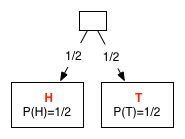
\includegraphics[width=2in]{figs/EventTree1Coin.png}
\end{center}
\caption{The event tree describing a single flip of a fair coin\label{fig:1Flip}}
\end{figure}

\section{Tossing a coin three times}

In this game the house tosses a fair coin three times in sequence. 
We consider different payment rules.

\begin{figure}[t]
\begin{center}
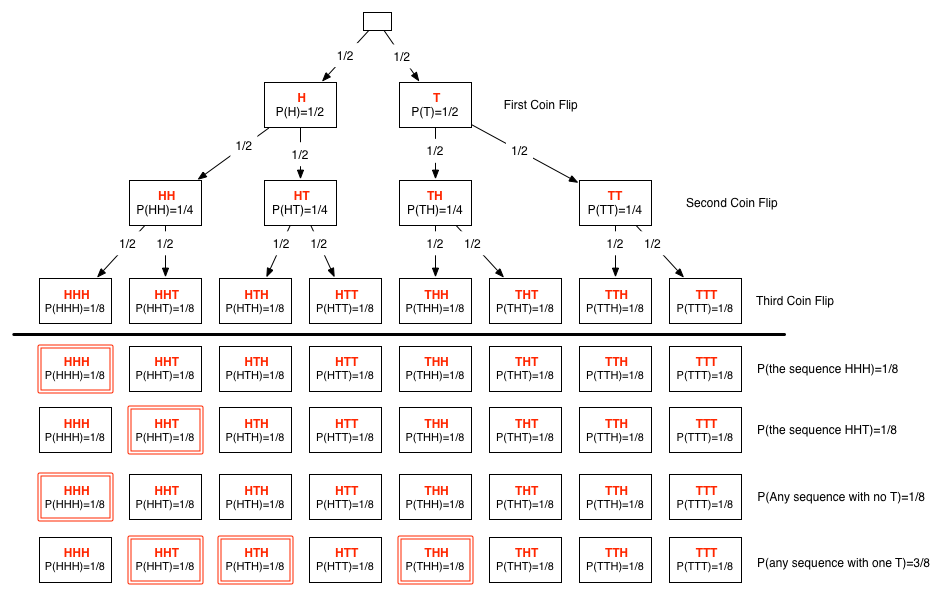
\includegraphics[width=6in]{figs/EventTree3Coins.png}
\end{center}
\caption{Event trees describing thre flips of a fair coin. {\bf (a)
    Specified outcome:} events of interests are HHH and HHT. {\bf (b)
    Number of tails:} events of interest are ``no tails'' (blue) and
  ``one tail'' (red). \label{fig:3Flips}}
\end{figure}

\subsection{Specific outcome}

The house pays one dollar if the outcome is HHH, nothing otherwise. What
is the fair price?

A single toss of a coin corresponds to two outcomes: H and T, each of
which has the same probability: $1/2$. A sequence of three tosses
generates a sequence of three letters, of which there are eight: TTT,
TTH, THT, THH, HTT, HTH, HHT, HHH. As each coin toss has probabilities
(1/2,1/2) and as they are {\em independent}~\footnote{We will define
  independence precisely later in the book. For now, it suffices to
  use the intuition that the outcome of each of the three coin tosses
  does not effect the other two.} we have that the probability of each
of the eight outcomes is $1/8$. We call the eight possible outcomes
the {\em outcome space}. As all eight outcomes have equal probability
we say that the distribution over the outcomes is {\bf uniform}.

As the player gets 1\$ when the outcome is HHH and nothing otherwise,
the expected gain, which is the fair ticket price, is 
$\frac{1}{8}(1+0+0+0+0+0+0+0)=\frac{1}{8}$.

Obviously, the same answer holds for any other sequence of 3
outcomes. For example for HHT.

\subsection{Specified number of tails}

Suppose that instead of specifying the sequence we specify the number
of times that Tails occured. Is that different from specifying the
sequence of outcomes? This depends on the specified number.

Suppose first that the number of tails is zero. There is only one
sequence that satisfies this condition, the sequence HHH. Thus the
probability of zero tails is $1/8$, and the fair price for the game is
an eighth of a dollar or 12.5 cents.

Next, suppose that the number of tails is {\bf one}. There are three
sequences that satisfy this condition: HHT,HTH,HHT. The probability of
a single tail is therefor three times larger than the probability of
each and the fair price for the game is $3/8 = 0.375$ or 37.5 cents.

Can you calculate the fair price for getting 1\$ if there are two
tails and if there are three tails?

We call the set of outcomes for which the game is won an {\em
  event}. Note the difference between an event and an outcome. An
outcome is a single outcome, an event is a {\em set} of outcomes that
can contain zero, one or more outcomes. In the next class we will discuss
sets and how they are used to calculate the probabilities of events.

\section{The three cards problem}

We finish this chapter with a slightly more complex example. The goal
of this example is to demonstrate the importance of having a
mathematical foundation and not relaying solely on intuition.

Consider the betting game. The house has three cards: one card is red
on both sides, one card is black on both sides and one card is black
on one side and red on the other side. We denote the three cards by
the letter pairs: BB,BR,RB.

The house choses one of the cards at random and puts it down on the
table with a randomly chosen side facing up.

Suppose the face up side is black. The house makes the following
offer: if the other side of the card is red, then the house will give
you a dollar, if the other side is black, you give the house a dollar.

If the side facing up is red, then the reverse offer is made: if the
other side is black, the house will give you a dollar, otherwise you
give the house a dollar.

The house claims the game is fair - say the face up side is black,
then there are two possible cards: BB and RB. As both of these cards
are equally likely to be chosen, the probabilities that the other side
is black or red are both $1/2$ and the game is fair.

Sounds convincing? It turns out that this is a false argument. The
truth is that the probability that the other side has the same color
is $2/3$ while the probability that it has the opposite color is
$1/3$. Thus the expected gain of the house is $2/3-1/3=1/3$. The house
gains a third of a dollar in expectation for each game!

How do we arrive at this answer? We need to carefully define the event
tree and the outcome space. To aid the explanation, study the event
tree in Figure~\ref{fig:3cards}. The event tree has two levels, the
first corresponding to the choice of card, the second to the choice of
card side. As a result, we get {\bf six} possible outcomes, each with
probability $1/6$. Note that there are {\bf two} outcomes
corresponding to the two sides of each card, depending on which side
of the card is facing up, as denoted by the up arrow: $\wedge$. This is
obvious for the card RB. It might be less obvious for the cards RR and
BB, because both sides of the card have the same color. However, the
two sides are obviously distinct, just imagine that we marked one side
of each card using invisible ink.

The rest of the argument is simple. Consider Figure~\ref{fig:3cards}
again. Suppose the face up side of the chosen card is red. There are
three outcomes that correspond to this event. Restricting our
attention to these three outcomes, we see that two correspond to the
card RR and one corresponds to the card RB. Thus the probability that
the bottom side is red {\bf ``conditioned''} on the fact that the
top card is red is $2/3$. This type of probability is called
``conditional'' probability. Conditional probability will play an
important role in following chapters.

\begin{figure}[t]
\begin{center}
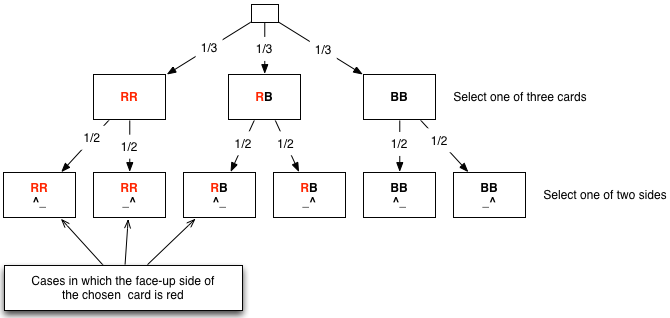
\includegraphics[width=4.5in]{figs/EventTree3Cards.png}
\end{center}
\caption{{\bf event tree describing the three cards problem.} The six
  nodes at the bottom level represent the six elements of the outcome
  space. The arrow up symbol $\wedge$ points to the side of the card
  that is facing up.\label{fig:3cards}}
\end{figure}

\section{Chapter Summary}
In this chapter we have discussed the following concepts. The
discussion was intuitive. In later chapters we will define the concepts
more precisely and use them to solve more complex problems.
\begin{itemize}
\item Outcomes.
\item Events.
\item Event tree.
\item Probabilities, probability distribution.
\item Uniform distribution.
\item Expected value, expectation, fair price.
\item Conditional probability.
\end{itemize}
